\documentclass[acmsmall]{acmart}
\microtypesetup{expansion=false} % local-compile safeguard (bitmap fallback fonts); harmless on Overleaf
% Same template and journal style as the author's mid-semester survey (ACM CSUR, acmsmall)
\acmJournal{CSUR}
\acmYear{2026}\acmVolume{1}\acmNumber{1}\acmArticle{}\acmMonth{11}
\setcopyright{none}
\settopmatter{printacmref=false}
\renewcommand\footnotetextcopyrightpermission[1]{}
\usepackage{booktabs}
\usepackage{array}
\newcolumntype{L}[1]{>{\raggedright\arraybackslash}p{#1}}
\usepackage{subcaption}
\usepackage{tikz}
\usetikzlibrary{positioning,arrows.meta,fit}
% AUTO-GENERATED by scripts/make_tables.py from results/*.csv -- do not edit
\newcommand{\NDocs}{61,877}
\newcommand{\NQueries}{54}
\newcommand{\NLists}{34}
\newcommand{\NJudg}{2,305}
\newcommand{\NPostJudg}{973}
\newcommand{\NTestAct}{35}
\newcommand{\NTestStale}{9}
\newcommand{\NTune}{10}
\newcommand{\NTuneAct}{7}
\newcommand{\NActive}{42}
\newcommand{\NStale}{12}
\newcommand{\MedRel}{30}
\newcommand{\TuneBMRpost}{0.094}
\newcommand{\TuneBMnDCG}{0.126}
\newcommand{\TuneGuard}{0.106}
\newcommand{\TuneBestFiniteRpost}{0.045}
\newcommand{\TuneBestFiniteH}{96}
\newcommand{\BMRpost}{0.146}
\newcommand{\BMnDCG}{0.187}
\newcommand{\BMRpre}{0.078}
\newcommand{\DFRpost}{0.181}
\newcommand{\DFdRpost}{$+$0.035}
\newcommand{\DFdRpostCI}{[$+$0.015, $+$0.058]}
\newcommand{\DFdnDCG}{$-$0.019}
\newcommand{\DFdnDCGCI}{[$-$0.039, $-$0.001]}
\newcommand{\DFpRpost}{0.005}
\newcommand{\DecdRpost}{$-$0.099}
\newcommand{\DecdRpostCI}{[$-$0.135, $-$0.068]}
\newcommand{\DecdnDCG}{$-$0.135}
\newcommand{\DecdnDCGCI}{[$-$0.177, $-$0.094]}
\newcommand{\TFdRpost}{$-$0.037}
\newcommand{\TFdnDCG}{$-$0.022}
\newcommand{\RecdRpost}{$-$0.133}
\newcommand{\RecdnDCG}{$-$0.178}
\newcommand{\StaleBMnDCG}{0.110}
\newcommand{\CondDFdRpost}{$+$0.032 [$+$0.012, $+$0.055]}
\newcommand{\CondDFdnDCG}{$-$0.022 [$-$0.041, $-$0.005]}
\newcommand{\CondDecdRpost}{$-$0.111 [$-$0.149, $-$0.075]}
\newcommand{\CondDecdnDCG}{$-$0.143 [$-$0.187, $-$0.100]}
\newcommand{\CondBMRpost}{0.167}
\newcommand{\NListsWindowEarly}{20}
\newcommand{\BMPostShare}{0.83}
\newcommand{\RelPostShare}{0.73}
\newcommand{\CorpusPostShare}{0.52}
\newcommand{\TFPostShare}{0.76}
\newcommand{\RatioTwenty}{0.88}
\newcommand{\RatioHundred}{0.73}
\newcommand{\DecayFacTwelve}{0.19}
\newcommand{\DecayFacNinetySix}{0.81}
\newcommand{\Growth}{3.9}
\newcommand{\ShareTwentyFiveCorpus}{0.23}
\newcommand{\ShareTwentyFiveDecay}{0.998}
\newcommand{\ShareTwentyFiveBM}{0.35}
\newcommand{\ShareTwentyFiveRel}{0.098}
\newcommand{\RhoDF}{0.46}
\newcommand{\RhoDFp}{0.005}
\newcommand{\RhoDec}{0.13}
\newcommand{\RhoDecp}{0.46}
\newcommand{\NDFHelps}{9}
\newcommand{\NDFHurts}{11}
\newcommand{\NDecHurts}{28}
\newcommand{\NDecHelps}{2}
\newcommand{\SensNinetySixRpost}{0.110}
\newcommand{\LatBM}{9.4}
\newcommand{\LatDec}{13.0}
\newcommand{\LatTF}{19.1}
\newcommand{\LatRec}{19.6}
\newcommand{\LatDF}{9.1}
\newcommand{\GrowthG}{0.157}
\newcommand{\GrowthRtwo}{0.96}
\newcommand{\GrowthGAbs}{0.180}
\newcommand{\DoublingYears}{4.4}
\newcommand{\GEighteen}{0.21}
\newcommand{\GTwentyNine}{0.32}
\newcommand{\GEighteenReview}{0.12}
\newcommand{\RhoTwenty}{0.146}
\newcommand{\RhoHundred}{0.345}
\newcommand{\NAllEighteen}{4,759}
\newcommand{\NAllTwentyFive}{14,697}

\makeatletter\let\inputtab\@@input\makeatother
\newcommand{\Rpost}{\mathrm{R}_{\text{post}}@20}
\newcommand{\TODO}[1]{\textbf{[TO VERIFY: #1]}}

\begin{document}

\title{Does Recency-Aware Re-ranking Close the Temporal Coverage Gap?}
\subtitle{A Controlled Retrieval-Stage Study for LLM-Assisted Literature Reviews}

\author{Himanshu Singh}
\affiliation{%
  \institution{[Institute] \textendash{} AI Tools for Research, enrollment MDE\_015}
  \country{India}}

\begin{abstract}
Large language models (LLMs) that draft literature reviews have a knowledge cutoff, and retrieval augmentation is the usual remedy for work published after it. Our earlier survey argued that this remedy is incomplete and that the share of post-cutoff literature a review actually covers has never been measured. This paper isolates one testable step of that argument: the retrieval stage. We ask whether re-ranking lexical search results by recency raises the coverage of papers published after a nominal cutoff $T$ (2023-07-01). We built a reproducible testbed from public sources. The corpus holds \NDocs{} ACL Anthology papers (2018--2025) with abstracts and dates. Relevance labels are \NJudg{} human-curated paper-list entries drawn from \NLists{} GitHub reading lists maintained by survey authors, which yield \NQueries{} topic queries. Topics were split by source list into tuning and held-out test sets, and the protocol was frozen before any run. We compared BM25, TF-IDF, a recency-only control, a hard date filter and BM25 with exponential time decay. The pre-registered tuning step rejected every finite decay half-life, so the proposed re-ranker reduced to BM25. Post hoc, every half-life lowered both post-cutoff recall ($\Rpost$) and nDCG@20 on the test topics; at $h=12$ months the paired change in $\Rpost$ was \DecdRpost{} \DecdRpostCI. A hard date filter raised $\Rpost$ by \DFdRpost{} \DFdRpostCI, below our pre-set threshold of $+0.05$, and it cost \DFdnDCG{} nDCG@20. It reduced nDCG to zero on topics with no recent literature. Plain BM25 was already skewed toward recent work: \BMPostShare{} of its top-20 results post-date $T$, against \RelPostShare{} of the curated relevant papers. Failure analysis shows that recency weighting floods rankings with the newest papers, which the curated lists themselves cover poorly. The ground truth therefore has a cutoff of its own. On this testbed, BM25's post-cutoff recall at depth 20, the survey's $\rho$, is only \RhoTwenty, and ACL output grows at $g=\GrowthG$ per year. These results suggest that retrieval-stage recency weighting is not a cheap fix for temporal coverage in LLM-written reviews, and that coverage evaluations need their own freshness checks.
\end{abstract}

\begin{CCSXML}
<ccs2012>
<concept><concept_id>10002951.10003317.10003338</concept_id><concept_desc>Information systems~Retrieval models and ranking</concept_desc><concept_significance>500</concept_significance></concept>
<concept><concept_id>10002951.10003317.10003359</concept_id><concept_desc>Information systems~Evaluation of retrieval results</concept_desc><concept_significance>500</concept_significance></concept>
<concept><concept_id>10010147.10010178.10010179.10010182</concept_id><concept_desc>Computing methodologies~Natural language generation</concept_desc><concept_significance>300</concept_significance></concept>
</ccs2012>
\end{CCSXML}
\ccsdesc[500]{Information systems~Retrieval models and ranking}
\ccsdesc[500]{Information systems~Evaluation of retrieval results}
\ccsdesc[300]{Computing methodologies~Natural language generation}

\keywords{knowledge cutoff, retrieval-augmented generation, temporal information retrieval, literature review automation, BM25, evaluation with incomplete judgments, negative result}

\maketitle

%=====================================================================
\section{Introduction}\label{sec:intro}
Our mid-semester survey \cite{ownreview2026} argued three things. A language model's knowledge cutoff is a graded boundary rather than a date, and the effective cutoff lies earlier than the reported one \cite{cheng2024dated} (survey \S4.1, Eq.~1). The cost of the boundary grows with the publication velocity of the field (\S4.2, Eq.~2--4). And the dominant failure in LLM-written reviews is \emph{omission} of recent work, which current evaluation practice barely measures (\S7.1). Unassisted models fabricate 18--55\% of citations \cite{walters2023fabrication}, and when asked to rebuild the reference lists of systematic reviews they reach at most 13.7\% recall \cite{chelli2024hallucination}. Retrieval augmentation \cite{lewis2020rag} and agentic literature systems \cite{shao2024storm,asai2026openscholar,skarlinski2024paperqa2,wang2024autosurvey} are the standard mitigation. The survey still traced four residual exposures through a retrieval-augmented review pipeline (\S5.1, Fig.~6). L1: queries inherit the model's vocabulary. L2: the index has its own latency and coverage bias. L3: evidence quantity and order matter. L4: parametric priors fill gaps. The survey concluded that retrieval does not close the gap. It also proposed the missing measurement: a \emph{temporal coverage ratio} $\mathrm{TCR}=|C\cap K_{post}|/|K_{post}|$, the share of essential post-cutoff work that a generated review cites (gap G1, direction D1, Eq.~5).

This paper turns one part of that argument into an experiment. We do not evaluate full generated reviews: that would need model access and expert reading lists we could not verify (Section~\ref{sec:limits}). Instead we study the \emph{retrieval stage} that feeds a review generator: the ``retrieval index $\rightarrow$ evidence selection'' step of the survey's Fig.~6. We hold query wording (L1) and index freshness (L2) fixed, so only the ranking changes. Its post-cutoff recall is exactly the quantity $\rho$ in the survey's temporal risk index $R=G(g,\Delta)(\lambda+\kappa)[1-\rho(1-\theta)]$ (Eq.~4). The survey noted that $\rho$ ``is measurable against a reference list'' but had no measurement of it. A natural engineering response to ``the model misses recent papers'' is to bias retrieval toward recency. Temporal information retrieval has long done this with time-based document priors \cite{li2003timebased,campos2014survey}. We test whether that response raises the retrieval-stage analogue of TCR without harming topical relevance.

\paragraph{Research questions.}
\textbf{RQ1} (intervention): On held-out topics, does BM25 with exponential time decay retrieve a larger fraction of relevant post-cutoff papers in the top 20 ($\Rpost$) than date-unaware BM25?
\textbf{RQ2} (trade-off): How do recency-enforcing controls (a hard ``published after $T$'' filter and pure recency sorting) trade post-cutoff recall against overall ranking quality and pre-cutoff recall?
\textbf{RQ3} (sensitivity and failure): How do the conclusions depend on the decay strength, on the cutoff date, and on how much of a topic's literature is recent? Where and why does recency weighting fail?

\paragraph{Contributions.} (i) A reproducible, fully public testbed for temporal coverage at the retrieval stage. It is built from ACL Anthology metadata and human-curated GitHub reading lists, pinned to commits. (ii) A pre-registered, controlled comparison with two lexical baselines, two recency controls and the decay re-ranker, plus sensitivity, cutoff-robustness, velocity, efficiency and failure analyses. (iii) Measured values for two quantities in the survey's severity model, the retrieval recall $\rho$ (Eq.~4) and a field growth rate $g$ (Eq.~3). (iv) A negative result with a mechanism: recency decay hurts. Lexical retrieval over a fast-growing corpus is already recency-skewed, and curated ground truth lags the newest literature. We claim no new algorithm. The contribution is the controlled evidence and the testbed.

%=====================================================================
\section{Background and Related Work}\label{sec:related}
\paragraph{Knowledge cutoffs.} Cheng et al.\ show that effective cutoffs often differ from reported ones because of stale material in web crawls and deduplication \cite{cheng2024dated}. FreshQA shows that search augmentation helps on fast-changing questions and that the number and order of retrieved evidence matter \cite{vu2023freshllms}. RealTime QA shows that models revert to outdated answers when retrieval is insufficient \cite{kasai2023realtimeqa}. These results concern question answering. Our survey argued that review writing is harder because its errors are omissive and retrieval is unbounded (survey \S4.4).

\paragraph{LLM literature synthesis and citation reliability.} Walters and Wilder found that 55\% (GPT-3.5) and 18\% (GPT-4) of citations in short model-written reviews were fabricated \cite{walters2023fabrication}. Chelli et al.\ compared LLM-generated reference lists for 11 systematic reviews (471 references) against the reviews' own lists. They report hallucination rates of 39.6\% (GPT-3.5), 28.6\% (GPT-4) and 91.4\% (Bard), and recall of 11.9\% and 13.7\% for the GPT models \cite{chelli2024hallucination}. Models can sometimes detect their own fabricated references through consistency checks \cite{agrawal2024references}. Retrieval-grounded and agentic systems such as STORM \cite{shao2024storm}, OpenScholar \cite{asai2026openscholar}, PaperQA2 \cite{skarlinski2024paperqa2} and AutoSurvey \cite{wang2024autosurvey} reduce fabrication by citing retrieved papers. Their coverage of recent work is therefore bounded by what the retriever ranks highly. The survey noted that none of them is evaluated against the set of important recent works it should have found (survey \S5.3). That is the stage we isolate. Gao et al.\ survey the wider RAG design space, including re-ranking \cite{gao2023ragsurvey}.

\paragraph{Temporal IR.} Li and Croft added an exponential recency prior to language-model retrieval for queries that favour recent documents \cite{li2003timebased}. Campos et al.\ survey later temporal ranking work \cite{campos2014survey}. Our decay re-ranker is the multiplicative analogue of that prior applied to BM25 \cite{robertson2009bm25}. It is a deliberately simple, transparent intervention, not a new method.

\paragraph{Evaluation with incomplete judgments.} Test collections rarely judge every relevant document. Buckley and Voorhees showed that standard measures are not robust to substantially incomplete judgments \cite{buckley2004incomplete}, and Sakai proposed evaluating condensed lists \cite{sakai2007bpref}. Our labels come from curated lists, so they are incomplete by construction. Section~\ref{sec:failure} shows that the incompleteness is \emph{time-dependent}, which matters for recency methods.

\begin{table}[t]
\caption{From the author's survey \cite{ownreview2026} to this experiment. Section, equation and figure numbers (\S, Eq., Fig.) refer to the survey; D0xx are entries of our decision log.}\label{tab:bridge}
\small
\begin{tabular}{@{}L{0.31\linewidth}L{0.35\linewidth}L{0.28\linewidth}@{}}
\toprule
Survey evidence & Operationalisation here & Status \\
\midrule
G1 (\S8.1), D1 (\S8.2): temporal coverage never measured; TCR $=|C\cap K_{post}|/|K_{post}|$ (Eq.~5) & $\Rpost$ with $C=$ top-20 retrieved and $K_{post}=$ curated papers dated $\geq T$ & Measured at the retrieval stage, not in generated reviews \\
$\rho$, recall of retrieval on post-cutoff work (Eq.~4) & BM25 $\mathrm{R}_{\text{post}}@k$ on test topics & Estimated: \RhoTwenty{} ($k{=}20$), \RhoHundred{} ($k{=}100$) (\S\ref{sec:linkback}) \\
Residual exposures L1--L4 (\S5.1, Fig.~6); retrieval cannot be evaluated in isolation (\S7.4) & Fixed corpus, human-fixed queries; only the ranker varies & Ranking isolated; L1 (G4, $\theta$) deliberately not varied \\
Velocity drives severity; $g$ values in Fig.~5 lack a source (\S4.2, Eq.~2--3; D008) & Growth of ACL Anthology output 2018--2025; topic post-cutoff share & $g=\GrowthG$/yr measured (\S\ref{sec:linkback}); velocity correlates with filter gains (\S\ref{sec:velocity}) \\
Benchmarks decay (\S7.2) & Curated reading lists as ground truth & Observed: labels lag the newest papers (\S\ref{sec:failure}) \\
Refresh GPT-3.5/4 anchors (\S7.6; D007) & -- & Not done: no verified model/API access (\S\ref{sec:limits}) \\
\bottomrule
\end{tabular}
\end{table}

%=====================================================================
\section{Study Design}\label{sec:method}
Table~\ref{tab:bridge} links the design to the survey. The protocol (\texttt{configs/experiment.json}) was frozen before any retrieval or evaluation was run. Figure~\ref{fig:pipeline} shows the pipeline.

\begin{figure}[t]
\centering
\resizebox{\linewidth}{!}{%
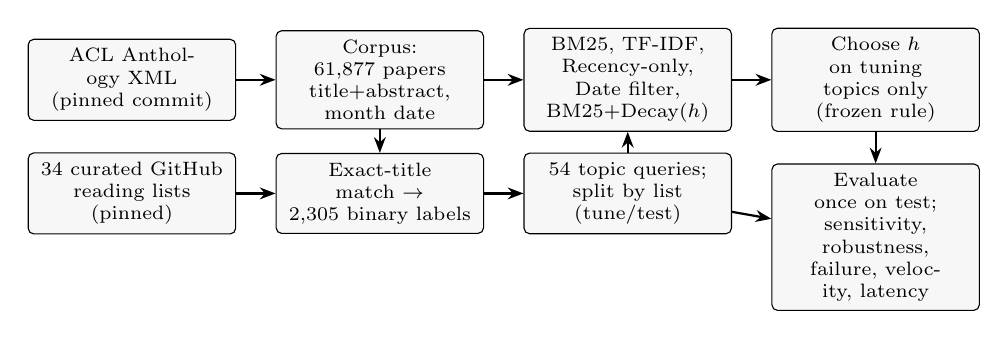
\begin{tikzpicture}[node distance=4mm and 5mm, every node/.style={font=\scriptsize, align=center},
  box/.style={draw, rounded corners=2pt, minimum height=8mm, text width=24mm, fill=gray!6},
  arr/.style={-{Stealth[length=2mm]}, thick}]
\node[box] (acl) {ACL Anthology XML\\(pinned commit)};
\node[box, below=of acl] (lists) {34 curated GitHub\\reading lists (pinned)};
\node[box, right=of acl] (corpus) {Corpus: \NDocs{} papers\\title+abstract, month date};
\node[box, right=of lists] (labels) {Exact-title match $\rightarrow$\\\NJudg{} binary labels};
\node[box, right=of labels] (queries) {\NQueries{} topic queries;\\split by list (tune/test)};
\node[box, right=of corpus] (methods) {BM25, TF-IDF, Recency-only,\\Date filter, BM25+Decay($h$)};
\node[box, right=of methods] (select) {Choose $h$ on tuning\\topics only (frozen rule)};
\node[box, below=of select] (eval) {Evaluate once on test;\\sensitivity, robustness,\\failure, velocity, latency};
\draw[arr] (acl) -- (corpus); \draw[arr] (lists) -- (labels); \draw[arr] (corpus) -- (labels);
\draw[arr] (labels) -- (queries); \draw[arr] (corpus) -- (methods); \draw[arr] (queries) -- (methods);
\draw[arr] (methods) -- (select); \draw[arr] (select) -- (eval); \draw[arr] (queries) -- (eval);
\end{tikzpicture}}
\Description{Pipeline from data sources to frozen evaluation.}
\caption{Experimental pipeline. Rankings are produced without access to labels; the decay half-life is chosen on tuning topics and the test topics are evaluated once.}\label{fig:pipeline}
\end{figure}

\subsection{Corpus}
We parsed the official ACL Anthology XML metadata \cite{aclanthology} at a pinned commit. We kept every paper from 2018--2025 that has a title and an abstract: \NDocs{} papers, out of 67,888 seen; 6,011 lacked abstracts. A paper's date is the first day of its volume's month. For 698 papers (1.1\%) the month is missing, so the date is set to 1 July of that year. The corpus grows quickly: 2025 has \Growth$\times$ as many papers as 2018 (Figure~\ref{fig:growth}). Rapidly growing fields are the setting in which the survey expected cutoffs to hurt most.

\subsection{Relevance labels from curated reading lists}
The survey's direction D1 proposes evaluating TCR on a panel of fields with expert-maintained reading lists, as a proxy for $K_{post}$; we follow that proposal. We used \NLists{} public GitHub repositories in which survey authors or research groups maintain topic-organised paper lists. Examples cover knowledge editing, hallucination, retrieval-augmented generation, long-context modelling, dialogue and machine translation. Each repository is pinned to a commit in \texttt{configs/lists.json}. A list entry counts as a relevant label only when the \emph{exact normalised title} of an Anthology paper (lower-case alphanumeric tokens, $\geq 4$ tokens) occurs in the entry line. This matching favours precision over recall: papers known only by arXiv titles that differ from their Anthology titles are missed. Twelve matched entries map to more than one Anthology record, and all such records are kept.

\paragraph{Queries.} For each list, or for a topical section of a broad list, we wrote one short topic query before any run, e.g.\ ``knowledge editing for large language models''. The query texts were drafted with AI assistance and are fixed in \texttt{configs/queries\_spec.json}. Queries with fewer than 8 relevant papers were dropped, leaving \NQueries{} queries and \NJudg{} labels (median \MedRel{} per query). A query is \emph{active} if at least 3 of its relevant papers are dated $\geq T$ (\NActive{} queries) and \emph{stale} otherwise (\NStale{}). Stale topics, such as event extraction and neural machine translation, are lists that stopped growing before $T$. They test whether recency methods harm topics whose literature is not recent.

\paragraph{Cutoff and split.} The nominal cutoff is $T=$ 2023-07-01, near the middle of the corpus window and in the period of the GPT-4-era anchors that the survey flagged as dating quickly (survey \S7.6). We also report $T=$ 2022-07-01 and 2024-07-01. Topics were split \emph{by source list} with a fixed seed, so that sections curated by the same group never appear in both sets. This gave \NTune{} tuning queries (\NTuneAct{} active) and 44 test queries (\NTestAct{} active, \NTestStale{} stale).

\subsection{Methods}
All methods index title+abstract with one tokenizer (lower-case \texttt{[a-z0-9]+}, no stemming), taken from the AI-generated starter code.
\begin{itemize}
\item \textbf{BM25} (primary baseline): Okapi BM25 with Lucene-style idf $\log(1+\frac{N-n_t+0.5}{n_t+0.5})$ and $k_1=0.9$, $b=0.4$, the Anserini defaults \cite{yang2017anserini,robertson2009bm25}. It ignores dates.
\item \textbf{TF-IDF} (second baseline): scikit-learn TF-IDF with cosine similarity \cite{pedregosa2011sklearn}.
\item \textbf{Recency-only} (control): the BM25 top-1000 candidates sorted newest first.
\item \textbf{Date filter} (control): BM25 restricted to papers dated $\geq T$. This is the ``since $T$'' filter of scholarly search engines and the most direct way to make retrieval cover what the model cannot know.
\item \textbf{BM25+Decay} (intervention): the BM25 top-1000 re-scored as
\begin{equation}\label{eq:decay}
s_h(q,d)=s_{\text{BM25}}(q,d)\cdot 2^{-a(d)/h},
\end{equation}
where $a(d)$ is the paper's age in months at $t_{\text{ref}}=$ 2025-12-01 and $h$ is a half-life. Here $h=\infty$ recovers BM25 exactly; we checked that the top-100 lists are identical. The grid $h\in\{3,6,12,24,48,96,\infty\}$ months was fixed in advance.
\end{itemize}

\subsection{Metrics, selection rule and statistics}
Let $R_q$ be the curated relevant set, $R_q^{post}=\{d\in R_q: t(d)\geq T\}$ and $R_q^{pre}=R_q\setminus R_q^{post}$. The primary metric is
\begin{equation}\label{eq:rpost}
\mathrm{R}_{\text{post}}@k(q)=\frac{|\mathrm{top}_k(q)\cap R_q^{post}|}{|R_q^{post}|},
\end{equation}
which is the survey's TCR (Eq.~5) evaluated on the retrieved set with $k=20$; averaged over topics it is also an estimate of the survey's $\rho$ (Eq.~4) for a given retriever and depth. Secondary metrics are binary nDCG@20 over $R_q$, pre-cutoff recall $\mathrm{R}_{\text{pre}}@20$, P@20 and median latency. Papers that are not on a list count as non-relevant; Section~\ref{sec:failure} examines this convention. Higher is better for every metric except latency.

\emph{Selection rule (frozen):} choose the $h$ that maximises mean $\Rpost$ on tuning active queries, subject to mean nDCG@20 $\geq$ BM25's $-0.02$.
\emph{Success criterion (frozen):} a mean paired gain in $\Rpost$ of at least $+0.05$ on test active queries, with a 95\% bootstrap CI excluding zero, and an nDCG@20 drop of at most 0.02. Uncertainty is reported as 95\% percentile CIs from 10,000 paired bootstrap resamples over queries (seed 2026) \cite{efron1993bootstrap}. Wilcoxon signed-rank $p$-values are given as descriptive support only, since 35 queries and many tied differences limit formal testing.

\subsection{Baseline validation}\label{sec:validation}
Before any comparison was run, we checked the following (validation log 03 in the repository).
(i) On a 3-document toy corpus, the sparse BM25 matches an independent loop implementation and a hand-computed value (0.493374).
(ii) On the full corpus, the two implementations agree to $3.6\times10^{-15}$ on three queries.
(iii) In a known-item test, each of 200 random titles used as a query returned its own paper at rank 1 in 194 cases and in the top 10 in all 200.
(iv) Our metric code reproduces hand-computed P, recall and nDCG on a toy ranking. On the real BM25 run it agrees with the AI-generated starter evaluator to $10^{-16}$ once the starter's input requirement is met (Section~\ref{sec:repro}).
(v) Twenty random label matches were printed and read; each matched Anthology title is on-topic for its list.
The baseline is our own implementation with Anserini's parameters. It is a validated comparator, not a numerical reproduction of a published run.

%=====================================================================
\section{Results}\label{sec:results}

\subsection{RQ1: the pre-registered selection rejects decay}
Table~\ref{tab:tuning} shows the tuning grid. On the \NTuneAct{} tuning active topics, every finite half-life lowered $\Rpost$ below BM25's \TuneBMRpost; the best finite value was \TuneBestFiniteRpost{} at $h=\TuneBestFiniteH$. Every finite half-life also failed the nDCG guardrail (BM25 \TuneBMnDCG; guardrail \TuneGuard). The frozen rule therefore selected $h^{*}=\infty$, and the intervention reduces to BM25 on the test set. H1 is \textbf{not supported}: the proposed re-ranker gives no gain because the protocol would not deploy it.

\begin{table}[t]
\caption{Tuning topics (\NTuneAct{} active): mean $\Rpost$ and nDCG@20 per half-life. Only $h=\infty$ passes the guardrail.}\label{tab:tuning}
\small
\begin{tabular}{@{}lccc@{}}
\toprule
$h$ (months) & $\Rpost$ & nDCG@20 & guardrail met \\
\midrule
\inputtab generated/tab_tuning.tex 
\bottomrule
\end{tabular}
\end{table}

\subsection{RQ1--RQ2 on held-out topics}
Table~\ref{tab:main} and Figure~\ref{fig:forest} report the \NTestAct{} test active topics. The decay rows other than $h^{*}$ are post hoc: they were run with all other settings but were not chosen by the protocol.

\begin{table}[t]
\caption{Held-out test topics with post-cutoff literature ($n=\NTestAct$), $k=20$, $T=$ 2023-07-01. $\Delta$ = mean paired difference from BM25 with 95\% bootstrap CI.}\label{tab:main}
\footnotesize\setlength{\tabcolsep}{2pt}
\begin{tabular}{@{}lccccc@{}}
\toprule
Method & $\Rpost$ & $\Delta\Rpost$ [95\% CI] & nDCG@20 & $\Delta$nDCG@20 [95\% CI] & $\mathrm{R}_{\text{pre}}@20$ \\
\midrule
\inputtab generated/tab_main.tex 
\bottomrule
\end{tabular}
\end{table}

\begin{figure}[t]
\centering
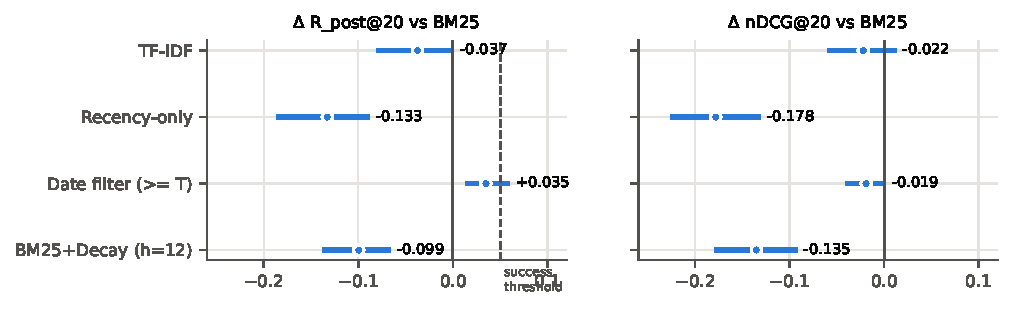
\includegraphics[width=\linewidth]{figures/fig_forest.pdf}
\Description{Paired differences from BM25 with confidence intervals.}
\caption{Paired differences from BM25 on test active topics (95\% bootstrap CIs). The dashed line marks the pre-registered success threshold for $\Delta\Rpost$.}\label{fig:forest}
\end{figure}

\paragraph{Observations.}
(1) \emph{Decay hurts.} At $h=12$ months, $\Rpost$ fell by \DecdRpost{} \DecdRpostCI{} and nDCG@20 by \DecdnDCG{} \DecdnDCGCI. nDCG fell on \NDecHurts{} of \NTestAct{} topics and rose on \NDecHelps. Recency-only sorting was worse still (\RecdRpost{} and \RecdnDCG).
(2) \emph{A hard date filter helps a little.} The filter raised $\Rpost$ from \BMRpost{} to \DFRpost{} (\DFdRpost{} \DFdRpostCI, Wilcoxon $p=\DFpRpost$), the only positive post-cutoff effect we observed. The gain is below the pre-registered $+0.05$ threshold, and nDCG@20 fell by \DFdnDCG{} \DFdnDCGCI. Pre-cutoff recall falls to zero by construction, so the filter only makes sense if pre-cutoff work is supplied some other way. That might be the model's parametric knowledge, a conjecture we did not test. The filter is therefore a promising control, not a demonstrated mitigation.
(3) \emph{TF-IDF is a weaker baseline than BM25} on both $\Rpost$ (\TFdRpost) and nDCG (\TFdnDCG).
(4) \emph{Absolute coverage is low for every method.} BM25 finds only \BMRpost{} of the curated post-cutoff papers in its top 20. The lists hold a median of \MedRel{} papers, so a perfect top-20 could not reach 1.0 for most topics. The gap nevertheless shows that topical precision, not recency, limits coverage at this stage.

\subsection{RQ2: harm on stale topics}
On the \NTestStale{} test topics without post-cutoff literature (Table~\ref{tab:stale}), the date filter, recency-only and decay at $h=12$ all lowered nDCG@20 from \StaleBMnDCG{} to 0. Recency enforcement is harmful when a user, or an LLM agent, asks about a field whose key work predates the cutoff.

\begin{table}[t]
\caption{Held-out stale topics ($n=\NTestStale$; no relevant paper dated $\geq T$).}\label{tab:stale}
\small
\begin{tabular}{@{}lccc@{}}
\toprule
Method & nDCG@20 & $\Delta$nDCG@20 [95\% CI] & P@20 \\
\midrule
\inputtab generated/tab_stale.tex 
\bottomrule
\end{tabular}
\end{table}

\subsection{RQ3: sensitivity to the decay half-life and to the cutoff}
Figure~\ref{fig:sens} sweeps $h$ on the test topics as a post hoc sensitivity analysis. Both metrics increase monotonically with $h$, and the plain BM25 limit is best on every curve. Even the gentlest decay ($h=96$ months, $\Rpost$ \SensNinetySixRpost) loses about a quarter of BM25's post-cutoff recall. Table~\ref{tab:cutoff} repeats the main comparison at three cutoffs. The direction of every effect holds. At $T=$ 2024-07-01 the date filter's gain is larger ($+0.047$), but so is its nDCG cost. The decay's loss in $\Rpost$ becomes uncertain at that cutoff (its CI includes 0), while its nDCG loss stays large.

\begin{figure}[t]
\centering
\begin{subfigure}[t]{0.49\linewidth}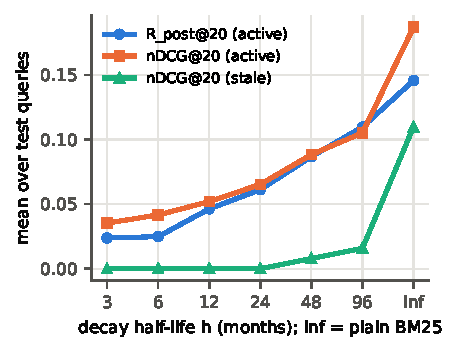
\includegraphics[width=\linewidth]{figures/fig_sensitivity.pdf}\caption{Decay half-life sweep (test topics, post hoc).}\label{fig:sens}\end{subfigure}\hfill
\begin{subfigure}[t]{0.49\linewidth}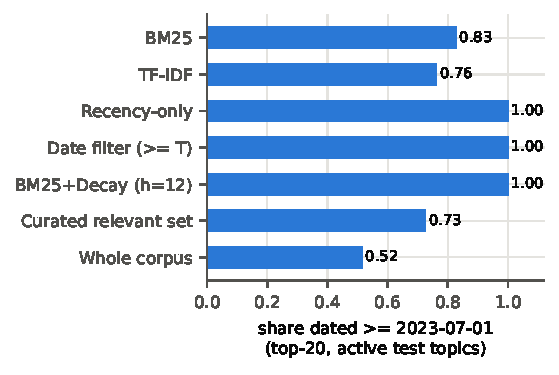
\includegraphics[width=\linewidth]{figures/fig_temporal_profile.pdf}\caption{Share of top-20 results dated $\geq T$.}\label{fig:profile}\end{subfigure}
\Description{Left: metrics rise with half-life. Right: BM25 top-20 is already mostly post-cutoff.}
\caption{(a) Every finite half-life is worse than plain BM25 ($h=\infty$). (b) BM25 already returns more post-cutoff papers (\BMPostShare) than the curated relevant sets contain (\RelPostShare) or the corpus holds (\CorpusPostShare).}
\end{figure}

\begin{table}[t]
\caption{Robustness to the cutoff date (test active topics; $n$ varies because activity depends on $T$). BM25 rows are absolute values; $\Delta$ rows are paired differences from BM25 [95\% CI].}\label{tab:cutoff}
\small
\begin{tabular}{@{}cclcc@{}}
\toprule
$T$ & $n$ & Row & $\Rpost$ & nDCG@20 \\
\midrule
\inputtab generated/tab_cutoff.tex 
\bottomrule
\end{tabular}
\end{table}

\subsection{Why decay fails: two mechanisms}\label{sec:failure}
\paragraph{Lexical retrieval is already recency-skewed.} Of BM25's top-20 results on test active topics, \BMPostShare{} are dated $\geq T$, against \RelPostShare{} of the curated relevant papers and \CorpusPostShare{} of the corpus (Figure~\ref{fig:profile}). A growing field produces more recent papers that match a topic's vocabulary, so date-unaware ranking already favours them. BM25 scores near the top are also compressed: the median score at rank 20 is \RatioTwenty{} of the rank-1 score, and at rank 100 it is \RatioHundred. Over the 29 months between $T$ and $t_{\text{ref}}$, the decay factor is \DecayFacTwelve{} at $h=12$ and \DecayFacNinetySix{} at $h=96$. Even the gentlest decay therefore outweighs most of the relevance signal within the top 100, and the ranking is decided by date. Under decay ($h=12$), \ShareTwentyFiveDecay{} of the top-20 results are from 2025, against \ShareTwentyFiveBM{} for BM25.

\paragraph{The ground truth has its own cutoff.} Only \ShareTwentyFiveRel{} of the curated relevant papers are from 2025, although 2025 holds \ShareTwentyFiveCorpus{} of the corpus. The lists lag the newest literature. Table~\ref{tab:example} shows the clearest case. For ``knowledge editing for large language models'', decay replaces the five listed papers in BM25's top 10 with ten November 2025 papers. Their titles are plainly about knowledge editing, but none is on the list. Such papers count as non-relevant here, so part of the measured loss is an artefact of stale labels. This is the survey's ``benchmarks decay'' (survey \S7.2) appearing in our own evaluation. To bound the artefact, we re-evaluated after removing, for each list, all papers dated after the list's newest relevant paper (a \emph{coverage-window} evaluation in the spirit of condensed lists \cite{sakai2007bpref}; \NListsWindowEarly{} of \NLists{} lists end before June 2025). The conclusions held. Decay changed $\Rpost$ by \CondDecdRpost{} and nDCG by \CondDecdnDCG; the date filter changed them by \CondDFdRpost{} and \CondDFdnDCG. This suggests that, even inside a list's coverage window, decay promotes recent papers that the curators did not list. Whether these papers are truly relevant can only be settled by human judgment \TODO{manually judge the top-20 of 3--5 topics}.

\begin{table}[t]
\caption{Top-10 for test query q01 (``knowledge editing for large language models''); \checkmark{} = on the curated list. Titles truncated.}\label{tab:example}
\scriptsize
\begin{tabular}{@{}L{0.48\linewidth}L{0.48\linewidth}@{}}
\toprule
BM25 (nDCG@20 = 0.471) & BM25+Decay, $h=12$ (nDCG@20 = 0.000) \\
\midrule
\checkmark{} 2024-08 WilKE: Wise-Layer Knowledge Editor & 2025-11 KELE: Residual Knowledge Erasure \\
\checkmark{} 2024-08 Cross-Lingual Knowledge Editing in LLMs & 2025-11 LyapLock: Bounded Knowledge Preserv. \\
\checkmark{} 2024-08 EasyEdit: \ldots Knowledge Editing Framework & 2025-11 GeoEdit: Geometric Knowledge Editing \\
2025-07 RuleEdit: Rule-Level Knowledge Generaliz. & 2025-11 Forget for Get: \ldots Knowledge Editing \\
2024-11 Editing the Mind of Giants: \ldots Pitfalls & 2025-11 M2Edit: Locate and Edit Multi-Granularity \\
\checkmark{} 2025-01 MLaKE: Multilingual Knowledge Editing & 2025-11 STEAM: Semantic-Level Knowledge Editing \\
2025-07 AdaEdit: Continuous Knowledge Editing & 2025-11 Can We Edit LLMs for Long-Tail Biomed.\ldots \\
\checkmark{} 2024-11 Knowledge Graph Enhanced LLM Editing & 2025-11 Side Effects of Rank-One Knowledge Editing \\
2024-08 DistillMIKE: Editing Distillation of \ldots & 2025-11 KoLEG: Korean Legal Knowledge Editing \\
2025-11 KELE: Residual Knowledge Erasure & 2025-11 MicroEdit: Neuron-level Knowledge \ldots \\
\bottomrule
\end{tabular}
\end{table}

\subsection{RQ3: topic velocity}\label{sec:velocity}
The survey predicted that cutoffs matter more in fast fields. As a velocity proxy we use the share of a topic's curated papers dated $\geq T$. Across test active topics, the date filter's nDCG gain rises with this share (Spearman $\rho=\RhoDF$, $p=\RhoDFp$, $n=\NTestAct$; Figure~\ref{fig:velocity}). The filter helped on \NDFHelps{} topics, mostly ones with high post-cutoff shares. It hurt on \NDFHurts{} topics, including five sub-topics from the dialogue and generation reading list and two RAG sub-topics, all with substantial pre-cutoff literature. Decay showed no such relation ($\rho=\RhoDec$, $p=\RhoDecp$). The proxy is computed from the labels themselves, so it describes the curated topic rather than the field, and the correlation is not causal.

\begin{figure}[t]
\centering
\begin{subfigure}[t]{0.49\linewidth}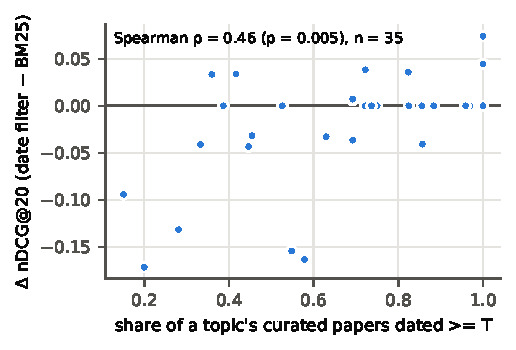
\includegraphics[width=\linewidth]{figures/fig_velocity.pdf}\caption{Date-filter gain vs.\ topic recency.}\label{fig:velocity}\end{subfigure}\hfill
\begin{subfigure}[t]{0.49\linewidth}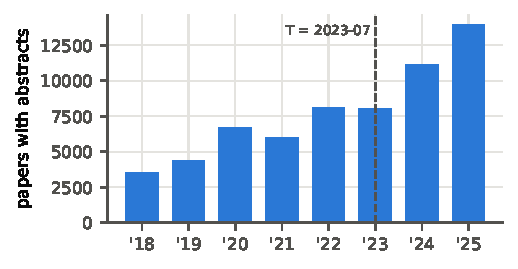
\includegraphics[width=\linewidth]{figures/fig_corpus_growth.pdf}\caption{Corpus papers per year.}\label{fig:growth}\end{subfigure}
\Description{Left: positive association between topic recency and date-filter gain. Right: corpus grows each year.}
\caption{(a) A hard date filter pays off only for topics whose literature is mostly post-cutoff. (b) The corpus grows \Growth$\times$ from 2018 to 2025.}
\end{figure}

\subsection{Linking back to the survey's severity model}\label{sec:linkback}
This analysis is post hoc and descriptive (\texttt{scripts/analysis\_growth.py}). The survey's unseen fraction $G(g,\Delta)=1-e^{-g\Delta}$ (Eq.~3) needs a growth rate $g$. Its Fig.~5 used $g=0.085$ for science at large \cite{bornmann2015growth} plus illustrative values of 0.20, 0.35 and 0.50 that had no cited source (decision D008). We fitted $\ln(\text{annual papers})$ on year for \emph{all} ACL Anthology papers from 2018 to 2025, which rise from \NAllEighteen{} to \NAllTwentyFive. The fit gives $g=\GrowthG$ per year ($R^2=\GrowthRtwo$), a doubling time of \DoublingYears{} years. Papers with abstracts give \GrowthGAbs, but abstract coverage improves over time, which inflates that figure. At $g=\GrowthG$, the survey's 18-month gap leaves $G\approx\GEighteen$ of the venue's literature unseen, against \GEighteenReview{} at the background rate. The 29-month gap from $T$ to $t_{\text{ref}}$ leaves $G\approx\GTwentyNine$. This is a whole-venue rate that also absorbs new tracks and workshops. LLM sub-topics, where 80--100\% of curated papers post-date $T$ (Figure~\ref{fig:velocity}), are clearly faster.

Our main metric also gives the survey's $\rho$. For BM25 on test topics, $\rho=\RhoTwenty$ at depth 20 and \RhoHundred{} at depth 100. Take the most favourable case for retrieval, with no terminological turnover ($\theta=0$, since our queries use current terms). The retrieval factor $[1-\rho(1-\theta)]$ of Eq.~4 is then 0.85 at depth 20 and 0.66 at depth 100. On this testbed, a lexical retriever that passes 20 papers to the generator removes only about 15\% of the survey's risk term, before any query staleness. Decay lowers $\rho$ (0.046 at $h=12$), and the date filter raises it only to 0.181. These values describe our queries, labels and corpus, not retrieval in general.

\subsection{Efficiency}
All methods run on a 2-core CPU with an in-memory sparse index; building the index takes about 7\,s. Median latency per query was \LatBM\,ms for BM25, \LatDF\,ms for the date filter, \LatDec\,ms for decay re-ranking, \LatTF\,ms for TF-IDF and \LatRec\,ms for recency sorting. Cost does not separate the methods; effectiveness does.

%=====================================================================
\section{Discussion}\label{sec:discussion}
\paragraph{Answers.} \emph{RQ1:} No. Under the frozen protocol, time decay was never selected, and every decay setting tested post hoc lowered post-cutoff recall and nDCG. \emph{RQ2:} Hard recency enforcement trades all pre-cutoff recall for a small, uncertain gain in post-cutoff recall ($+0.035$, below our threshold). That trade is acceptable only for topics whose literature is mostly recent. \emph{RQ3:} The decay result holds across half-lives and cutoffs, and the filter result depends on topic recency. Decay fails because lexical scores near the top are compressed and the corpus grows. Its measured harm is inflated, though not explained away, by ground truth that lags the newest papers.

\paragraph{What this means for the survey's argument.} The survey listed index lag, retrieval quality and query staleness as reasons why retrieval does not close the cutoff gap. With the index current and the queries written in current terminology, our data point to retrieval quality. BM25 already over-represents recent work, yet finds only about one in seven curated post-cutoff papers in its top 20. Pushing harder on recency trades relevance for novelty. Better topical relevance is the more promising lever, for example dense retrieval, or the citation-graph and index-derived query expansion that the survey proposed as D4. This is an inference that our data motivate but do not test. A second implication is methodological: anyone measuring TCR must check the freshness of the reference set. Otherwise a recent but stale benchmark will penalise exactly the systems that find recent work.

\paragraph{Alternative explanations.} (a) \emph{Query wording:} short topic queries favour generic matches. Longer or LLM-generated queries could change absolute levels, though both arms used the same queries. (b) \emph{Matching bias:} exact-title matching misses papers whose arXiv and Anthology titles differ, which may reduce recall uniformly. (c) \emph{List curation style:} some lists favour surveys or benchmarks, which BM25 matches well. (d) \emph{Date granularity:} month-level dates and the inclusive cutoff count July 2023 venues (e.g., ACL 2023) as post-cutoff.

%=====================================================================
\section{Threats to Validity and Limitations}\label{sec:limits}
\textbf{Construct validity.} Like the survey's own anchors (survey \S7.6), our numbers are tied to a dated snapshot and should be re-run as corpora and lists change (survey \S8.3). $\Rpost$ measures what a retriever surfaces, not what a generated review cites; we did not run an LLM generator. Turning this into a full test of review-level omission, and refreshing the Chelli-style replication (decision D007), needs model access and expert reference lists that we did not have verified access to. \textbf{Ground truth.} Curated lists are incomplete, unevenly maintained and time-lagged (Section~\ref{sec:failure}), and unlisted papers count as non-relevant. No human relevance judgments were collected. \textbf{External validity.} The corpus is one community's venues (ACL Anthology), and arXiv-only work is absent. Results may differ for biomedicine or for web-scale scholarly indexes. \textbf{Statistical.} There are 35 test active topics and 9 stale ones, the tuning set has only 7 active topics, and several topics share curators. The bootstrap resamples queries, not lists. \textbf{Selection.} Queries were drafted with AI assistance before any run. The decay grid, cutoff and thresholds were fixed in advance, while the coverage-window analysis, the mechanism analysis and the full-depth rankings were added after the tuning result and are labelled post hoc. \textbf{Novelty.} We did not run a systematic prior-art search, so no novelty is claimed beyond the specific controlled setting.

%=====================================================================
\section{Reproducibility and AI-Use Statement}\label{sec:repro}
The repository contains the code, frozen configs, pinned data sources and every result file. Re-running \texttt{scripts/run\_all.sh} regenerates all tables, figures and the number macros used in this paper (\texttt{paper/generated/}); no result is typed by hand. Retrieval is deterministic, with ties broken by paper ID, and bootstrap resampling uses seed 2026. The environment was Python 3.13.18 with pandas 3.0.5, NumPy 2.5.3, SciPy 1.18.1, scikit-learn 1.9.1 and Matplotlib 3.11.2 on CPU.
\emph{AI use.} An AI assistant generated the earlier planning documents and starter code (Prompts 03--14). In this session it wrote and ran the experiment code, drafted the queries and this manuscript, and verified bibliographic metadata. Three logged incidents shaped the final code. (1) The starter environment test failed because \texttt{rank\_bm25} was not installed and package installation was blocked, so BM25 was re-implemented and validated against an independent loop. (2) The starter evaluator refused to score any ranking containing unjudged papers (``4959 ranked query-paper pairs lack relevance labels''), so unjudged papers were treated as non-relevant and the metrics were cross-checked against the starter's code. (3) An unexpected collapse of recall under gentle decay was investigated as a possible bug and traced to the mechanism in Section~\ref{sec:failure}. The author must re-run the pipeline, check the code and judge the flagged items \TODO{author confirms re-run and review of code, queries and labels}.

%=====================================================================
\section{Conclusion}\label{sec:conclusion}
We tested a simple, popular idea for reducing knowledge-cutoff omissions in LLM-assisted literature reviews: biasing retrieval toward recent papers. Under a frozen protocol on a public testbed, exponential time decay never helped. A hard post-cutoff filter gave a small gain in post-cutoff coverage, below our success threshold, at the cost of all pre-cutoff work and of stale topics. Lexical retrieval over a growing literature is already recency-skewed, and curated ground truth trails the newest papers. Ranked by cost and expected information, three follow-ups remain. First, judge the top-20 of a few topics by hand to measure label staleness directly. Second, add a dense retriever under the same split. Third, run a small end-to-end generator to compute TCR on actual generated reviews.

\bibliographystyle{ACM-Reference-Format}
\bibliography{references}

\end{document}
